\begin{figure}
  \centering
  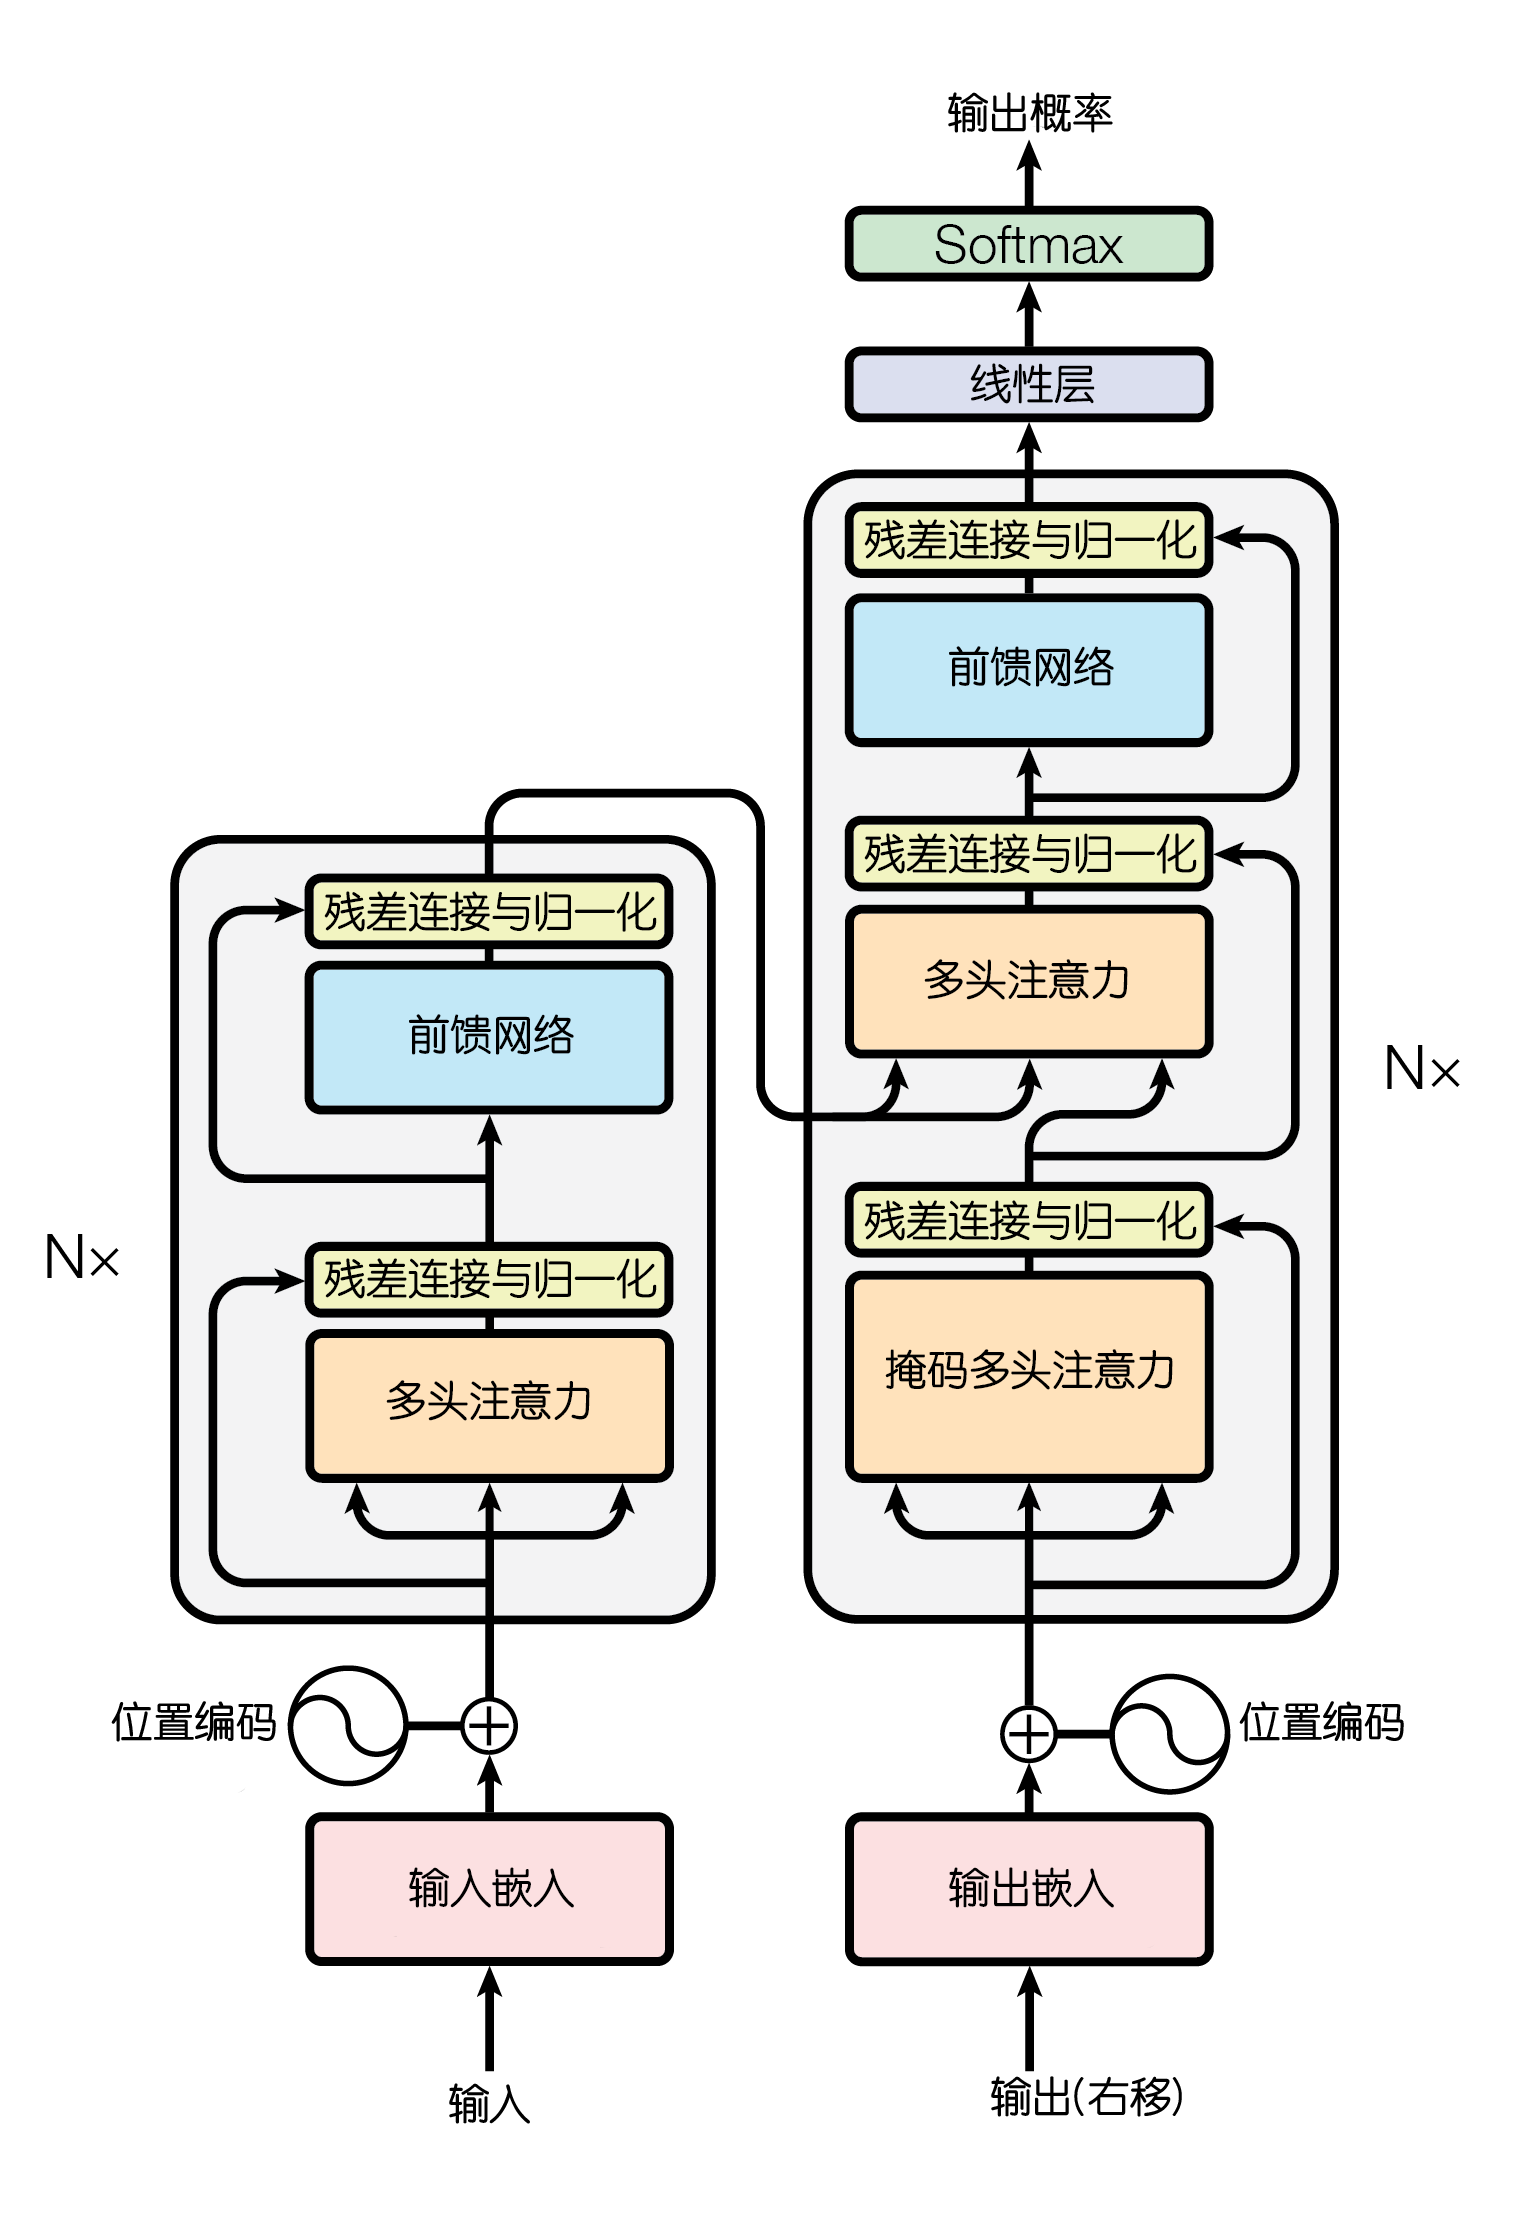
\includegraphics[scale=0.6]{Figures/ModalNet-21}
  \caption{Transformer 模型架构。}
  \label{fig:model-arch}
\end{figure}

% 尽管我们模型的主要组成部分是注意力,
% 我们的模型保持了编码器-解码器结构,这种结构在许多所谓的序列到序列模型中很常见 \citep{bahdanau2014neural,sutskever14}。与所有此类架构一样,编码器计算输入序列的表示,解码器消耗这些表示以及输出标记,以自回归的方式产生输出序列。传统上,编码器和解码器包含循环或卷积层堆叠,而我们的编码器和解码器堆叠由注意力层和逐位置前馈层组成(图~\ref{fig:model-arch})。以下章节详细描述了整体架构和这些特定组件。

大多数具有竞争力的神经序列转导模型都具有编码器-解码器结构 \citep{cho2014learning,bahdanau2014neural,sutskever14}。这里,编码器将符号表示的输入序列 $(x_1, ..., x_n)$ 映射到连续表示的序列 $\mathbf{z} = (z_1, ..., z_n)$。给定 $\mathbf{z}$,解码器然后一次一个元素地生成符号的输出序列 $(y_1,...,y_m)$。在每一步,模型是自回归的 \citep{graves2013generating},在生成下一个符号时消耗先前生成的符号作为额外输入。

Transformer 遵循这种整体架构,对编码器和解码器使用堆叠的自注意力和逐点全连接层,分别如图~\ref{fig:model-arch} 的左右半部分所示。

\subsection{编码器和解码器堆叠}

\paragraph{编码器:}编码器由 $N=6$ 个相同层堆叠而成。每层有两个子层。第一个是多头自注意力机制,第二个是简单的逐位置全连接前馈网络。我们在每个子层周围使用残差连接 \citep{he2016deep},然后进行层归一化 \cite{layernorm2016}。也就是说,每个子层的输出是 $\mathrm{LayerNorm}(x + \mathrm{Sublayer}(x))$,其中 $\mathrm{Sublayer}(x)$ 是子层本身实现的函数。为了促进这些残差连接,模型中的所有子层以及嵌入层都产生维度 $\dmodel=512$ 的输出。

\paragraph{解码器:}解码器也由 $N=6$ 个相同层堆叠而成。除了每个编码器层中的两个子层外,解码器插入第三个子层,该子层对编码器堆叠的输出执行多头注意力。与编码器类似,我们在每个子层周围使用残差连接,然后进行层归一化。我们还修改了解码器堆叠中的自注意力子层,以防止位置关注到后续位置。这种掩码结合输出嵌入偏移一个位置的事实,确保对位置 $i$ 的预测只能依赖于位置小于 $i$ 的已知输出。

% 在我们的模型(图~\ref{fig:model-arch})中,编码器和解码器由交替的自注意力层(用于跨位置通信)和逐位置前馈层(用于就地计算)堆叠而成。此外,解码器堆叠包含编码器-解码器注意力层。由于注意力对词之间的距离不可知,我们的模型需要向编码器和解码器输入添加“位置编码”。以下章节详细描述所有这些组件。

\subsection{注意力} \label{sec:attention}
注意力函数可以描述为将查询和一组键值对映射到输出,其中查询、键、值和输出都是向量。输出计算为值的加权和,其中分配给每个值的权重通过查询与相应键的兼容性函数计算。

\subsubsection{缩放点积注意力} \label{sec:scaled-dot-prod}

% \begin{figure}
%   \centering
%   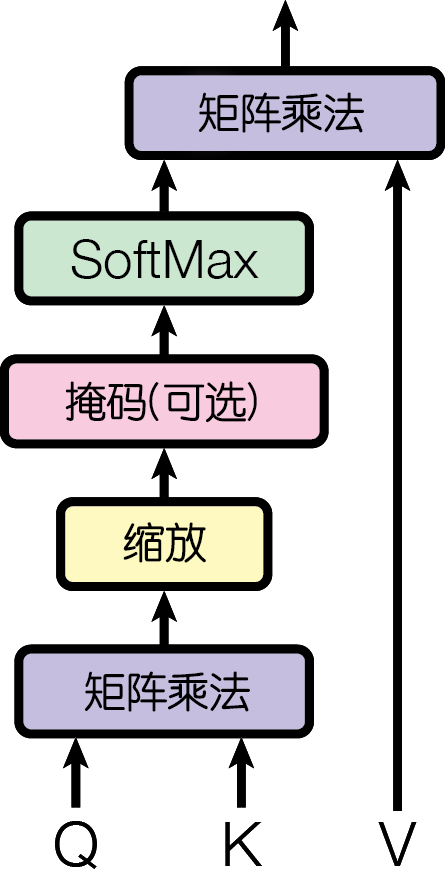
\includegraphics[scale=0.6]{Figures/ModalNet-19}
%   \caption{缩放点积注意力。}
%   \label{fig:multi-head-att}
% \end{figure}

我们将我们的特定注意力称为“缩放点积注意力”(图~\ref{fig:multi-head-att})。输入由维度 $d_k$ 的查询和键,以及维度 $d_v$ 的值组成。我们计算查询与所有键的点积,每个除以 $\sqrt{d_k}$,然后应用 softmax 函数来获得值的权重。

在实践中,我们同时计算一组查询的注意力函数,将它们打包成矩阵 $Q$。键和值也打包成矩阵 $K$ 和 $V$。我们计算输出矩阵为:

\begin{equation}
   \mathrm{Attention}(Q, K, V) = \mathrm{softmax}(\frac{QK^T}{\sqrt{d_k}})V
\end{equation}

两种最常用的注意力函数是加性注意力 \citep{bahdanau2014neural} 和点积(乘法)注意力。点积注意力与我们的算法相同,除了缩放因子 $\frac{1}{\sqrt{d_k}}$。加性注意力使用具有单个隐藏层的前馈网络计算兼容性函数。虽然两者在理论复杂度上相似,但点积注意力在实践中更快且更节省空间,因为它可以使用高度优化的矩阵乘法代码实现。

% 我们将点积缩放 $1/\sqrt{d_k}$ 以限制点积的幅度,这在实践中效果很好。否则,我们发现应用 softmax 通常会导致权重非常接近 0 或 1,从而产生极小的梯度。

% 已在后续章节描述
% 当用作解码器自注意力的一部分时,在 softmax 之前应用可选的掩码函数以防止位置关注到后续位置。该掩码简单地将所有非法连接(下三角外部)对应的 logits 设置为 $-\infty$。

%\paragraph{与加性注意力的比较:} 我们选择点积注意力而非加性注意力 \citep{bahdanau2014neural},因为它可以使用高度优化的矩阵乘法代码计算。这种优化对我们尤为重要,因为我们在模型中使用了许多注意力层。

虽然对于较小的 $d_k$ 值,两种机制表现相似,但对于较大的 $d_k$ 值,不加缩放的点积注意力不如加性注意力 \citep{DBLP:journals/corr/BritzGLL17}。我们怀疑对于较大的 $d_k$ 值,点积的幅度会变大,将 softmax 函数推入梯度极小的区域\footnote{为了说明点积为何变大,假设 $q$ 和 $k$ 的分量是均值为 $0$、方差为 $1$ 的独立随机变量。那么它们的点积 $q \cdot k = \sum_{i=1}^{d_k} q_ik_i$ 的均值为 $0$,方差为 $d_k$。}。为了抵消这种效应,我们将点积缩放 $\frac{1}{\sqrt{d_k}}$。

% 我们怀疑这是因为点积幅度变得过大,导致应用 softmax 函数后梯度无用。为了抵消这一点,我们将点积缩放 $1/\sqrt{d_k}$。

\subsubsection{多头注意力} \label{sec:multihead}

\begin{figure}
\begin{minipage}[t]{0.5\textwidth}
  \centering
  缩放点积注意力 \\
  \vspace{0.5cm}
  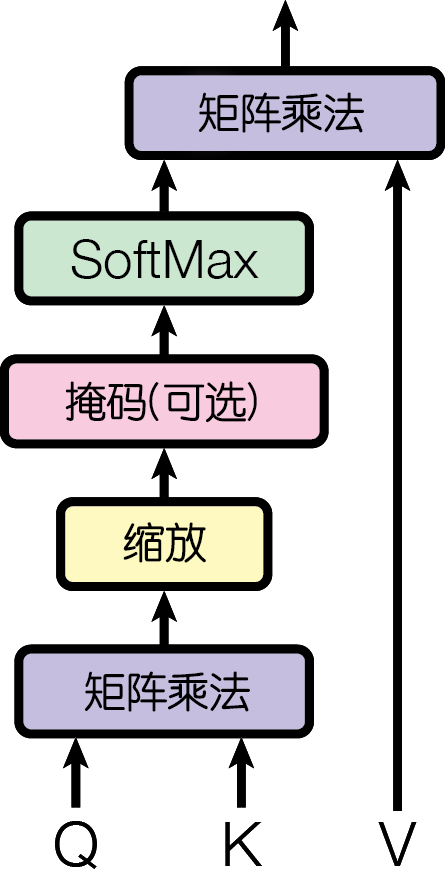
\includegraphics[scale=0.6]{Figures/ModalNet-19}
\end{minipage}
\begin{minipage}[t]{0.5\textwidth}
  \centering 
  多头注意力 \\
  \vspace{0.1cm}
  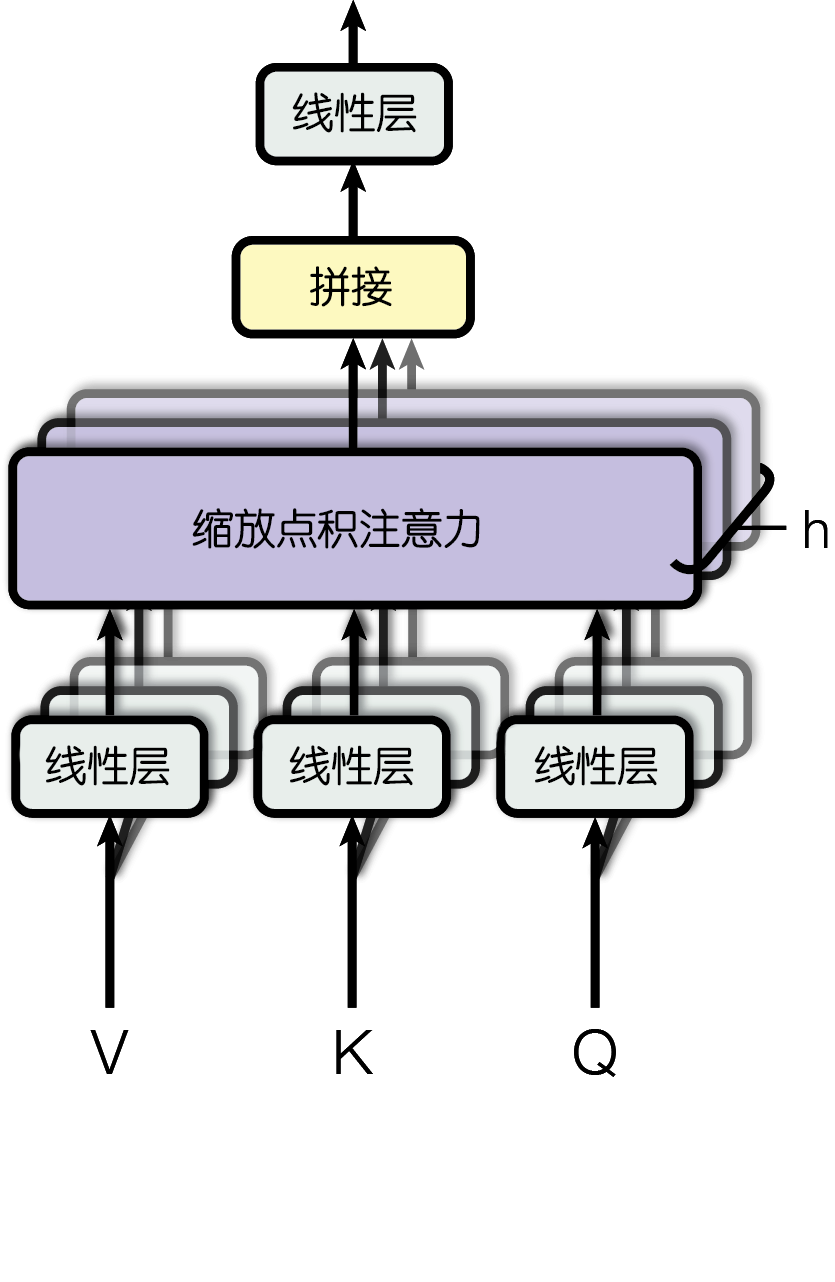
\includegraphics[scale=0.6]{Figures/ModalNet-20}  
\end{minipage}


  % \centering

  \caption{(左)缩放点积注意力。(右)多头注意力由几个并行运行的注意力层组成。}
  \label{fig:multi-head-att}
\end{figure}

我们发现,与使用 $\dmodel$ 维键、值和查询执行单个注意力函数相比,将查询、键和值用不同的学习线性投影线性投影 $h$ 次到 $d_k$、$d_k$ 和 $d_v$ 维度是有益的。
然后我们在这些投影版本的查询、键和值上并行执行注意力函数,产生 $d_v$ 维输出值。这些输出被连接并再次投影,得到最终值,如图~\ref{fig:multi-head-att} 所示。

多头注意力允许模型在不同位置联合关注来自不同表示子空间的信息。使用单个注意力头时,平均会抑制这一点。

\begin{align*}
    \mathrm{MultiHead}(Q, K, V) &= \mathrm{Concat}(\mathrm{head_1}, ..., \mathrm{head_h})W^O\\
%    \mathrm{where} \mathrm{head_i} &= \mathrm{Attention}(QW_Q_i^{\dmodel \times d_q}, KW_K_i^{\dmodel \times d_k}, VW^V_i^{\dmodel \times d_v})\\
    \text{其中}~\mathrm{head_i} &= \mathrm{Attention}(QW^Q_i, KW^K_i, VW^V_i)\\
\end{align*}

其中投影是参数矩阵 $W^Q_i \in \mathbb{R}^{\dmodel \times d_k}$, $W^K_i \in \mathbb{R}^{\dmodel \times d_k}$, $W^V_i \in \mathbb{R}^{\dmodel \times d_v}$ 和 $W^O \in \mathbb{R}^{hd_v \times \dmodel}$。

% 我们发现(且成本不更高)使用多个并行注意力层(每个层覆盖全部位置),其键、值和查询维度按比例降低更好。我们称之为“多头注意力”(图~\ref{fig:multi-head-att})。每个并行注意力层的键、值和查询通过对多头注意力的输入进行学习线性变换计算。我们在不同并行注意力层之间使用不同的线性变换。并行注意力层的输出被连接,然后通过最终的学习线性变换。

在这项工作中,我们使用 $h=8$ 个并行注意力层或头。对于每个头,我们使用 $d_k=d_v=\dmodel/h=64$。
由于每个头的维度减少,总计算成本与全维单头注意力相似。

\subsubsection{注意力在我们模型中的应用}

Transformer 在三个方面使用多头注意力:
\begin{itemize}
 \item 在“编码器-解码器注意力”层中,查询来自前一个解码器层,记忆键和值来自编码器的输出。这允许解码器中的每个位置关注输入序列中的所有位置。这模仿了序列到序列模型中的典型编码器-解码器注意力机制,例如 \citep{wu2016google, bahdanau2014neural,JonasFaceNet2017}。

 \item 编码器包含自注意力层。在自注意力层中,所有键、值和查询来自相同的地方,即编码器中前一层的输出。编码器中的每个位置可以关注编码器前一层中的所有位置。

 \item 类似地,解码器中的自注意力层允许解码器中的每个位置关注解码器中包括该位置在内的所有位置。我们需要防止解码器中的向左信息流以保持自回归特性。我们通过在 softmax 的输入中将所有对应非法连接的值掩码(设置为 $-\infty$)来实现这一点。见图~\ref{fig:multi-head-att}。

\end{itemize}

\subsection{逐位置前馈网络}\label{sec:ffn}

除了注意力子层外,编码器和解码器的每个层都包含一个全连接前馈网络,该网络分别且相同地应用于每个位置。这包括两个线性变换,中间有 ReLU 激活。

\begin{equation}
   \mathrm{FFN}(x)=\max(0, xW_1 + b_1) W_2 + b_2
\end{equation}

虽然线性变换在不同位置相同,但它们在层与层之间使用不同的参数。另一种描述方式是使用核大小为 1 的两个卷积。输入和输出的维度为 $\dmodel=512$,内层维度为 $d_{ff}=2048$。

% 在附录中,我们描述了逐位置前馈网络如何也可以被视为注意力的一种形式。

%来自 Jakob:模型关联两个任意输入或输出位置信号所需的操作数随输入或输出中位置之间的距离增长,对于 ConvS2S 线性增长,对于 ByteNet 对数增长,使得学习这些位置之间的依赖关系更加困难 \citep{hochreiter2001gradient}。在 Transformer 中,这减少为常数操作数,尽管代价是由于平均注意力加权位置导致的有效分辨率降低,我们旨在通过多头注意力抵消这种效应。

%图~\ref{fig:simple-att} 展示了一个简单的注意力函数 $A$,具有单个头,构成我们多头注意力的基础。$A$ 接受查询键向量 $\kq$、记忆键矩阵 $\km$ 和记忆值矩阵 $\vm$,并产生查询值向量 $\vq$ 作为
%\begin{equation*} \label{eq:attention}
%    A(\kq, \km, \vm) = {\vm}^T (Softmax(\km \kq).
%\end{equation*}
%在调用注意力函数之前,我们使用学习矩阵 ${\Wkq \text{,} \, \Wkm}$ 和 ${\Wvm}$ 线性变换 $\kq,\,\km$ 和 $\vm$,并在将其传递给前馈层之前使用 $\Wvq$ 变换输出查询。每个注意力层有自己的一组变换矩阵,这些矩阵在所有查询位置共享。$A$ 在每个查询位置并行应用,并作为矩阵乘法的批处理高效实现。自注意力和编码器-解码器注意力层使用 $A$,但参数不同。例如,在编码器自注意力中,编码器层 $i$ 中的查询关注编码器层 $i-1$ 中的记忆。为确保解码器自注意力层不查看未来词,我们为查询位置 $l$ 将位置 $j+1$ 到查询长度的 logits 添加 $- \inf$。

%在简单注意力中,查询值是记忆值的加权组合,其中注意力权重和为 1。尽管该函数在实践中表现良好,但注意力权重的约束可能限制从记忆到查询的信息流,因为查询不能同时关注多个记忆位置,这在翻译长序列时可能是可取的。\marginpar{@usz,你能想到一个例子吗?} 我们通过在每个查询位置维护多个注意力头来补救,这些头并行关注所有记忆位置,每个注意力头 $h$ 有不同参数集。
%\marginpar{}

\subsection{嵌入和 Softmax}
与其他序列转导模型类似,我们使用学习嵌入将输入标记和输出标记转换为维度 $\dmodel$ 的向量。我们还使用通常的学习线性变换和 softmax 函数将解码器输出转换为预测的下一个标记概率。在我们的模型中,我们在两个嵌入层和 softmax 前线性变换之间共享相同的权重矩阵,类似于 \citep{press2016using}。在嵌入层中,我们将这些权重乘以 $\sqrt{\dmodel}$。

\subsection{位置编码}
由于我们的模型不包含循环和卷积,为了使模型利用序列的顺序,我们必须注入关于序列中标记的相对或绝对位置的信息。为此,我们在编码器和解码器堆叠的底部向输入嵌入添加“位置编码”。位置编码具有与嵌入相同的维度 $\dmodel$,以便两者可以相加。位置编码有许多选择,学习的和固定的 \citep{JonasFaceNet2017}。

在这项工作中,我们使用不同频率的正弦和余弦函数:

\begin{align*}
    PE_{(pos,2i)} = sin(pos / 10000^{2i/\dmodel}) \\
    PE_{(pos,2i+1)} = cos(pos / 10000^{2i/\dmodel})
\end{align*}

其中 $pos$ 是位置,$i$ 是维度。也就是说,位置编码的每个维度对应一个正弦曲线。波长形成从 $2\pi$ 到 $10000 \cdot 2\pi$ 的几何级数。我们选择这个函数是因为我们假设它允许模型轻松学习通过相对位置关注,因为对于任何固定偏移 $k$,$PE_{pos+k}$ 可以表示为 $PE_{pos}$ 的线性函数。

我们还尝试使用学习的位置嵌入 \citep{JonasFaceNet2017},发现两个版本产生几乎相同的结果(见表~\ref{tab:variations} 行 (E))。我们选择正弦版本,因为它可能允许模型外推到训练期间遇到的序列长度更长的序列。
